%///////////////////////////////////////////////////////////////////////////////
% <file
%   repository_path  = "$Source: /pub/cvsprojects/nucleo/web/home/modules/libstatmech/doc/tex/screening.tex,v $"
%   revision         = "$Revision: 1.5 $"
%   date             = "$Date: 2009/08/27 02:18:16 $"
%   tag              = "$Name:  $"
%   template_version = "cp_template.0.12"
% >
%
% <license>
%   See the README_module.xml file for this module for copyright and license
%   information.
% </license>
%   <description>
%     <abstract>
%       This is the Webnucleo Report describing the screening example in the
%       libstatmech distribution.
%     </abstract>
%     <keywords>
%       libstatmech Module, webnucleo report
%     </keywords>
%   </description>
%
%   <authors>
%     <current>
%       <author userid="tyu" start_date="2009/08/18" />
%       <author userid="mbradle" start_date="2012/01/30" />
%     </current>
%     <previous>
%     </previous>
%   </authors>
%
%   <compatibility>
%     TeX (Web2C 7.4.5) 3.14159 kpathsea version 3.4.5
%   </compatibility>
%
% </file>
%///////////////////////////////////////////////////////////////////////////////
%
% This is a sample LaTeX input file.  (Version of 9 April 1986)
%
% A '%' character causes TeX to ignore all remaining text on the line,
% and is used for comments like this one.

\documentclass[pdftex]{article}    % Specifies the document style.

\usepackage[dvips]{graphicx}
\usepackage{hyperref}

                           % The preamble begins here.
\title{Webnucleo Technical Report: Screening Example with libstatmech}  % Declares the document's title.

\author{Tianhong Yu and Bradley S. Meyer}

\begin{document}           % End of preamble and beginning of text.

\maketitle                 % Produces the title.

This technical report describes some details of the screening example
in the libstatmech distribution.

\section{Thomas Fermi Screening}

The Thomas-Fermi model is a quantum mechanical theory for the electronic 
structure of many-body systems. For simplicity, we will just apply a Yukawa 
potential to the electrons in an atom to describe the screening effect. The 
example demonstrates how to add a user-defined potential to the integrand. 

The Yukawa potential is a function of radius away from a charge:
\[
\phi(r) = \frac{Ze}{r} e^{-r/r_0}
\]
where $Z$ is the atomic number, $e$ is the proton charge, $r_0$ is a parameter
to describe how the potential drops with radius.  Because the potential
contributes to the energy of an electron, the number density integral for
electrons in the presence of the charge becomes a function of the radius:
\[
n(r) = \frac {(mc^2)^3g} {2\pi^2(\hbar c)^3\gamma^3}
  \int_0^{\infty} (x+\gamma)\sqrt{x^2+2\gamma x}
  \left[
    \frac{1}{1+{\exp}(x - \mu'/kT - e\phi(r)/kT)}
  \right]
  \, dx
\]
\[
  \equiv
  \int_0^\infty n(r,x) \, dx
\]
\[
  \equiv
  n(r,T,\mu_{eff}/kT)
\]
where the effective chemical potential is
\[
\frac{\mu_{eff}}{kT} = \frac{\mu'}{kT} + \frac{e\phi(r)}{kT}.
\]

To find the chemical potential, we consider that the nuclei are separated
by a distance $2R$ and thus associate a sphere of radius $R$ with each
nucleus.  Because of charge neutrality, the average number density is
\[
\langle n_e \rangle = \frac{3Z}{4\pi R^3}.
\]
We similarly have the constraint
\[
\int_0^R 4 \pi r^2 n(r) \, dr = Z.
\]
We can thus define a number density
\[
n_e( T, \mu'/kT ) = \frac{3Z}{R^3} \int_0^R dr \, r^2 n_e(r,T,\mu_{eff}/kT)
\, dx.
\]
We use the integrand for $n_e( T, \mu'/kT )$ in the example.
$n_e( T, \mu'/kT )$ needs to
equal the average number density $\langle n_e \rangle$.

We use $e^2 = \alpha \hbar c$ in the example, where
$\alpha$ is the fine-structure constant, $\hbar$ is Planck's constant divided
by $2\pi$, and $c$ is the speed of light in vacuum.  We use the GNU
Scientific Library values for these constants (in cgs units).

\section{Example}

The figure below shows how the electron number density drops with 
radius under the Yukawa potential.  In general, the electrons are concentrated
towards the nucleus because of the Coulomb attraction.
The smaller the $r_0$ value, the more
the Coulomb potential from the nucleus is screened.  The electron number
density then flattens in the outer radii.

In running the examples, we found some cases, particularly at small temperature,
where the calculation did not converge.  Decreasing the integral accuracy
can solve this problem.  Commented code in the example shows how to do this.

\begin{figure}[htp]
\centering
\resizebox{\textwidth}{!}{
  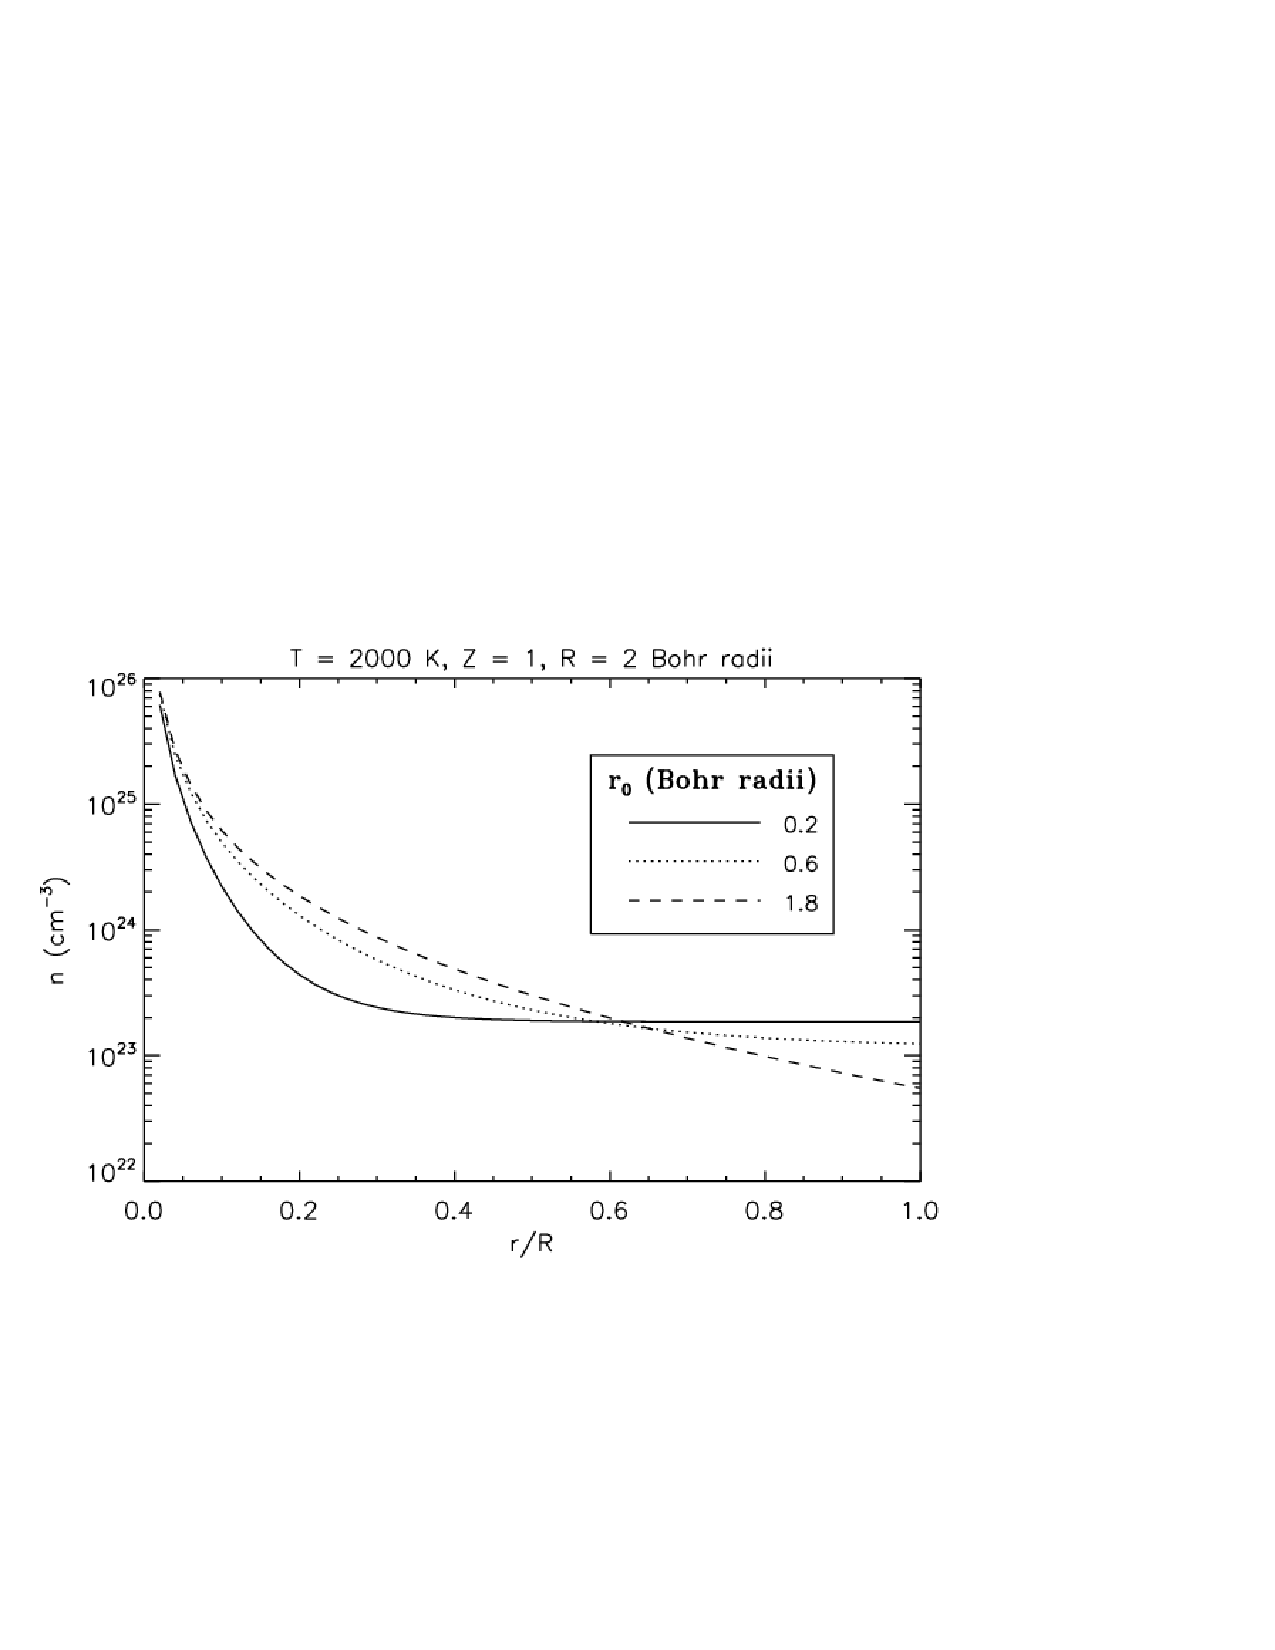
\includegraphics{figures/n_r.pdf}
  }
\caption{Number densities vs radius. For atomic number = 1 and atomic radius
  = 2 (Bohr radius), the electron densities get larger at smaller radius where
the Coulomb pull from the nucleus is higher.} 
\label{fig:n_r}
\end{figure}

\end{document}
